\documentclass[times,11pt]{ACME2015article}
\usepackage{amsmath,amssymb,amsthm,mathrsfs,graphicx}
\usepackage{natbib,subfigure}
\usepackage{titlesec}
\usepackage{wrapfig}

\setlength{\parindent}{0pt}
\setlength{\parskip}{5pt plus 2pt minus 1 pt}

\topmargin  -25mm
\evensidemargin 0mm
\oddsidemargin  0mm
\textwidth  160mm
\textheight 267mm
%\renewcommand{\baselinestretch}{1.0}
\frenchspacing
\sloppy
\titlespacing{\section}{0pt}{\parskip}{0.01\parskip}
%%%%%%%%%%%%%%%%%%%%%%%%%%%%%%%%%%%%%%%%%%%%%%%%%%%%%%%%%%%%%%%%%%%%%%%
\begin {document}
\pagestyle{empty}

\begin{flushright}
{\fontsize{8}{10}
\it Abstracts of the 23$^\mathrm{rd}$ UK Conference of the\\
Association for Computational Mechanics in Engineering\\
8 - 10 April 2015, Swansea University, Swansea\\} \vskip 1.2 cm
\end{flushright}

\begin{center}
{\fontsize{14}{20}\bf Computation of resonant modes in cavities with a Discontinuous Galerkin time domain approach
%
%   The title goes here...
%
}\end{center}


\begin{center}
\textbf{M. Dawson, R. Sevilla, O. Hassan and K. Morgan}\\
\end{center}

\begin{center}
{\fontsize{10}{12}
Zienkiewicz Centre for Computational Engineering, College of Engineering, Swansea University, Swansea, Wales, UK SA2 8PP\\
}\end{center}

\begin{center}
\{743587,R.Sevilla,O.Hassan,K.Morgan\}@swansea.ac.uk\\
\end{center}
%
\begin{center}
\textbf{ABSTRACT}\\[1mm]
\end{center}
%

\begin{normalsize}
Recent advances in manufacturing techniques, such as electron beam lithography, make it possible to manufacture devices on the scale of the wavelength of light. This has opened the doors to manipulation of light in novel new ways - such as....  In particular nanoscale resonators which have been demonstrated with well defined resonances and high quality factors. History, history, history.... Such resonators have many applications including for nanolasers optical circuitry and biological sensing. However, the typical scale and the geometric complexity introduce several challenges for numerical simulation.

\begin{wrapfigure}{r}{0.3\textwidth}
 \centering
 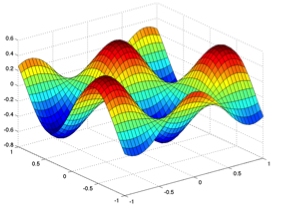
\includegraphics[width=0.25\textwidth]{DispersiveCavityPlot}
 \caption{A component of the electromagnetic field in a square cavity filled with a dispersive material.}
 \label{MicroToroidalSensor:graph}
\end{wrapfigure}

The majority of nanoscale devices at optical frequencies can be simulated using classical electromagnetism and disregarding quantum effects since ****. For metallic devices, the frequency dependence of material parameters becomes significant and should be accounted for using the Drude or Drude-Lorentz models, see an example of a computation in a dispersive cavity in Figure \ref{MicroToroidalSensor:graph}. Frequency domain solvers \cite{ref1} are traditionally employed to find the resonant frequencies and associated modes, but as the scale and geometric complexity of the devices increases, the large eigenvalue system that must be solved becomes computationally prohibitive.

We propose to use the Discontinuous Galerkin (DG) method with explicit time marching, which only requires solving a block diagonal system of equations for each time step \cite{ref2}. [ exand on why this is a better approach ] The resonant frequencies, quality factors and mode shapes can then be recovered by a periodic sampling of the solution in time using the Fast Fourier Transform or similar, more advanced, techniques. Quantities of interest, such as resonant frequencies, quality factors and mode shapes are then obtained from the spectrum by curve fitting.

Since the resolution and cutoff frequency depends on the number of timesteps taken in the simulation - long-running simulations are desirable to obtain desired accuracy. This is an additional benefit of the DG method since parallisation can be achieved in a relatively simple way - allowing good accuracy in reasonable computational time.

We discuss in detail the implementation of a parallelised DG electromagnetic solver, capable of full 3D simulation of dispersive metallic cavities. We present a study on the sampling rates and duration of the sampled signal required to obtain a given spectrum resolution. We validate the method by assessing the optical properties of resonators for problems with known solutions. Finally, we present results for a realistic metal-coated semiconductor nanocylinder resonator.

\begin{center}
\textbf{RESULTS}\\[1mm]
\end{center}

\begin{center}
\textbf{CONCLUSION}\\[1mm]
\end{center}

\end{normalsize}


\begin{thebibliography}{99}
\bibitem{ref1}
Busch, Kurt, Michael König, and Jens Niegemann. ``Discontinuous Galerkin methods in nanophotonics.'' Laser \& Photonics Reviews 5.6 (2011): 773-809.

\bibitem{ref2}
Sevilla, Ruben, Oubay Hassan, and Kenneth Morgan. ``The use of hybrid meshes to improve the efficiency of a discontinuous Galerkin method for the solution of Maxwell’s equations.'' Computers \& Structures 137 (2014): 2-13.

\end{thebibliography}

\end{document}